Diffie--Hellman (DH) protocol is a method of asymmetric exchange
of the cryptographic keys for a group of two or more participants,
developed in 1976 by cryptographers Ralph Merkle, Whitfield Diffie and Martin Hellman.
In contrast to the symmetric key exchange,
the Diffie\textendash Hellman protocol eliminates the direct transfer of the shared secret
between the participants so that each participant computes a shared secret with his own private-public key pair.
The Diffie\textendash Hellman protocol is based on a one-way function of the form

\begin{equation}
    A = G ^ a \bmod P \label{eq:equation}
\end{equation}

where $A$ is the user's public key,
$a$ is the user's private key,
$P=2Q+1$ is modulus, such that 2048 bits safe-prime because $Q$ is also prime,
$G$ is generator such that $G$ is primitive root modulo $P$.
We say that $G$ is primitive root modulo $P$ if for each $1 \leq a \leq P - 1$ the $A = G ^ a \bmod P$
is unique and belong to the set $\{1, 2, \dots, P-1\}$.
The period of such cyclic group $\mathbb{Z}_{P}$ is $P-1$ then.

Thus, the safety of the Diffie--Hellman protocol is based on the \textbf{discrete logarithm problem} which is unsolvable
in polynomial time if the constants $G$ and $P$ are chosen correctly.
Graphically the flow of the Diffie--Hellman protocol can be expressed through the
analogy with mixing paints as the picture below shows
\begin{figure}[H]
    \centering
    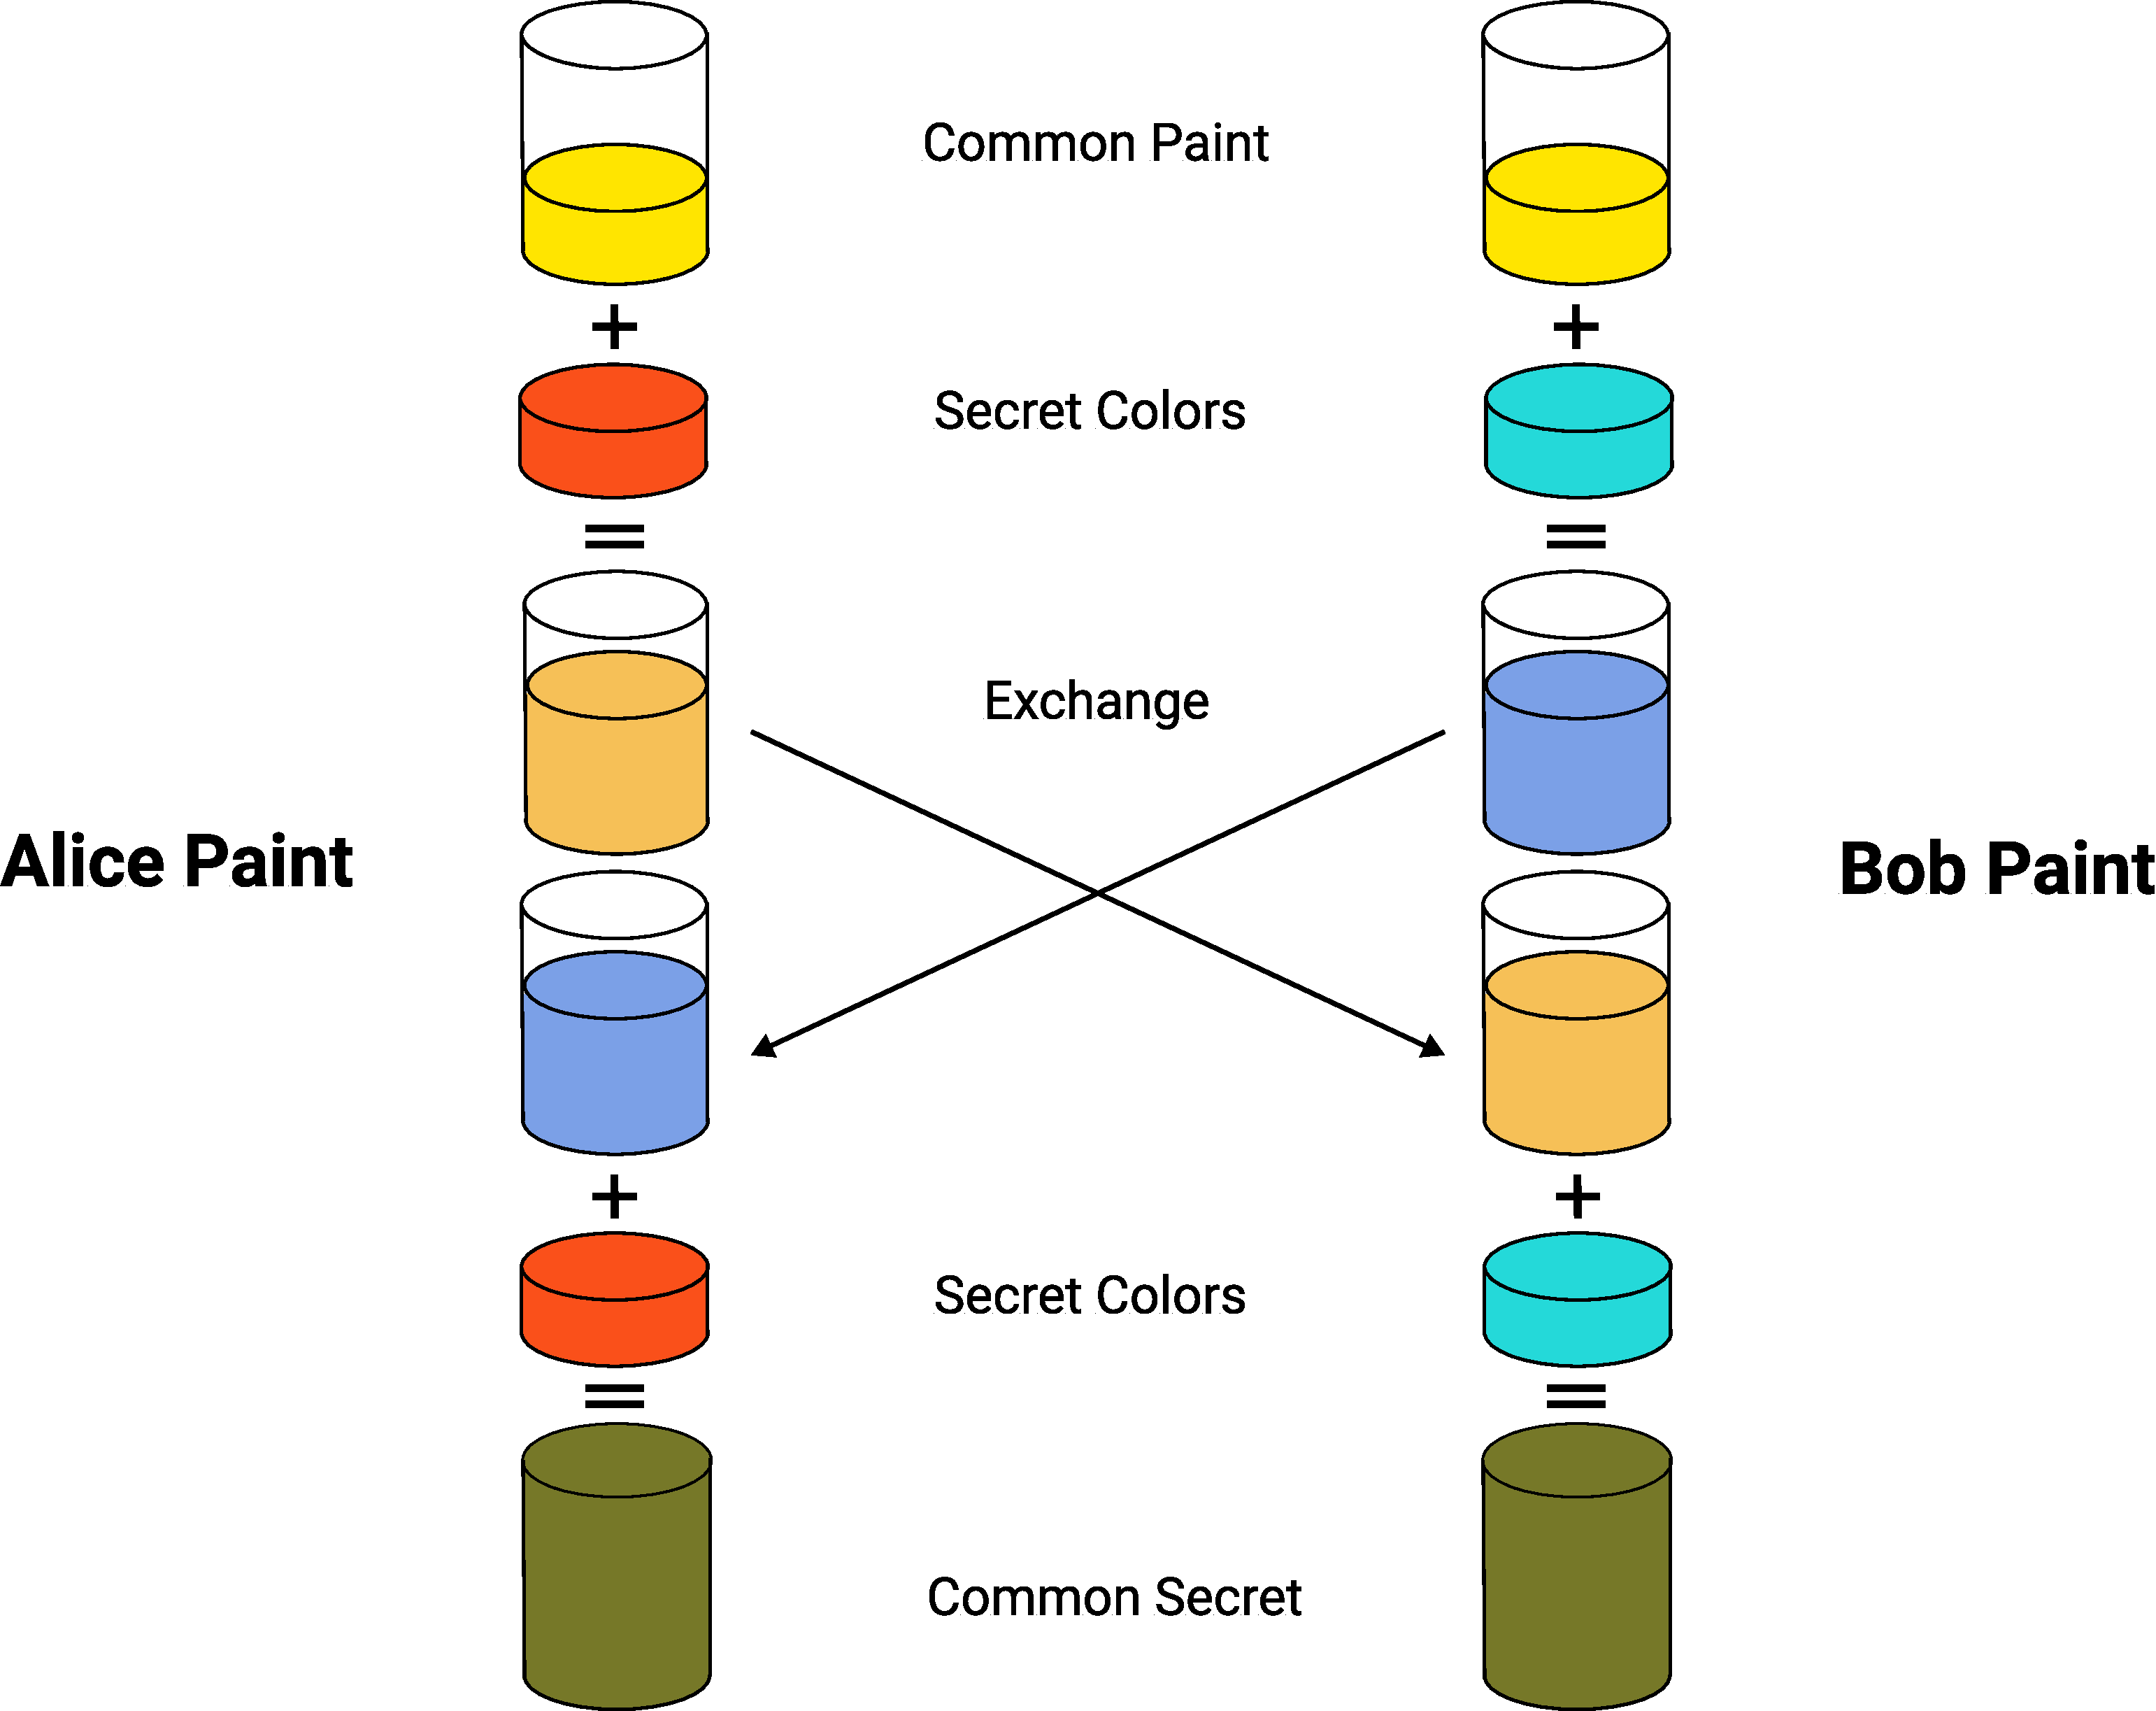
\includegraphics[width=1\textwidth]{Pictures/Diffie_Hellman_keyexchange_concept_diagram}
    ~\caption{Diffie\textendash Hellman key exchange concept diagram.}\label{fig:figure4}
\end{figure}
In contrast to the Diffie\textendash Hellman based on discrete logarithm problem,
there is an Elliptic Curve Diffie\textendash Hellman key exchange which is based on the elliptic curve discrete logarithm problem.
Although, the idea is quite similar, the difference only in that Elliptic Curve Diffie\textendash Hellman ensures the same safety
as discrete logarithm Diffie\textendash Hellman with lower number of bits of the prime modulus $P$.
For instance, 521 bit modulus used in Elliptic Curve Diffie\textendash Hellman is equally safe as 2048 bit modulus in
discrete logarithm Diffie\textendash Hellman.
To summarize, the flow of Diffie\textendash Hellman key exchange is as follows.
Given 2048 bits public prime modulus $P$ and generator $G$ such that $G$ is primitive root modulo $P$ then
\begin{enumerate}
    \item Alice chooses her secret $a$.
    \item Alice sends to Bob her public key $A = G^a \bmod P$.
    \item Bob chooses his secret $b$.
    \item Bob sends to Alice his public key $B = G^b \bmod P$.
    \item Alice computes common secret $s = B^a \bmod P$.
    \item Bob computes common secret $s = A^b \bmod P$.
    \item Alice and Bob have arrived to the same value
    \begin{align}
        s = A^b \bmod P = G^{ab} \bmod P \\
        s = B^a \bmod P = G^{ba} \bmod P
    \end{align}
\end{enumerate}

\begin{figure}[H]
    \centering
    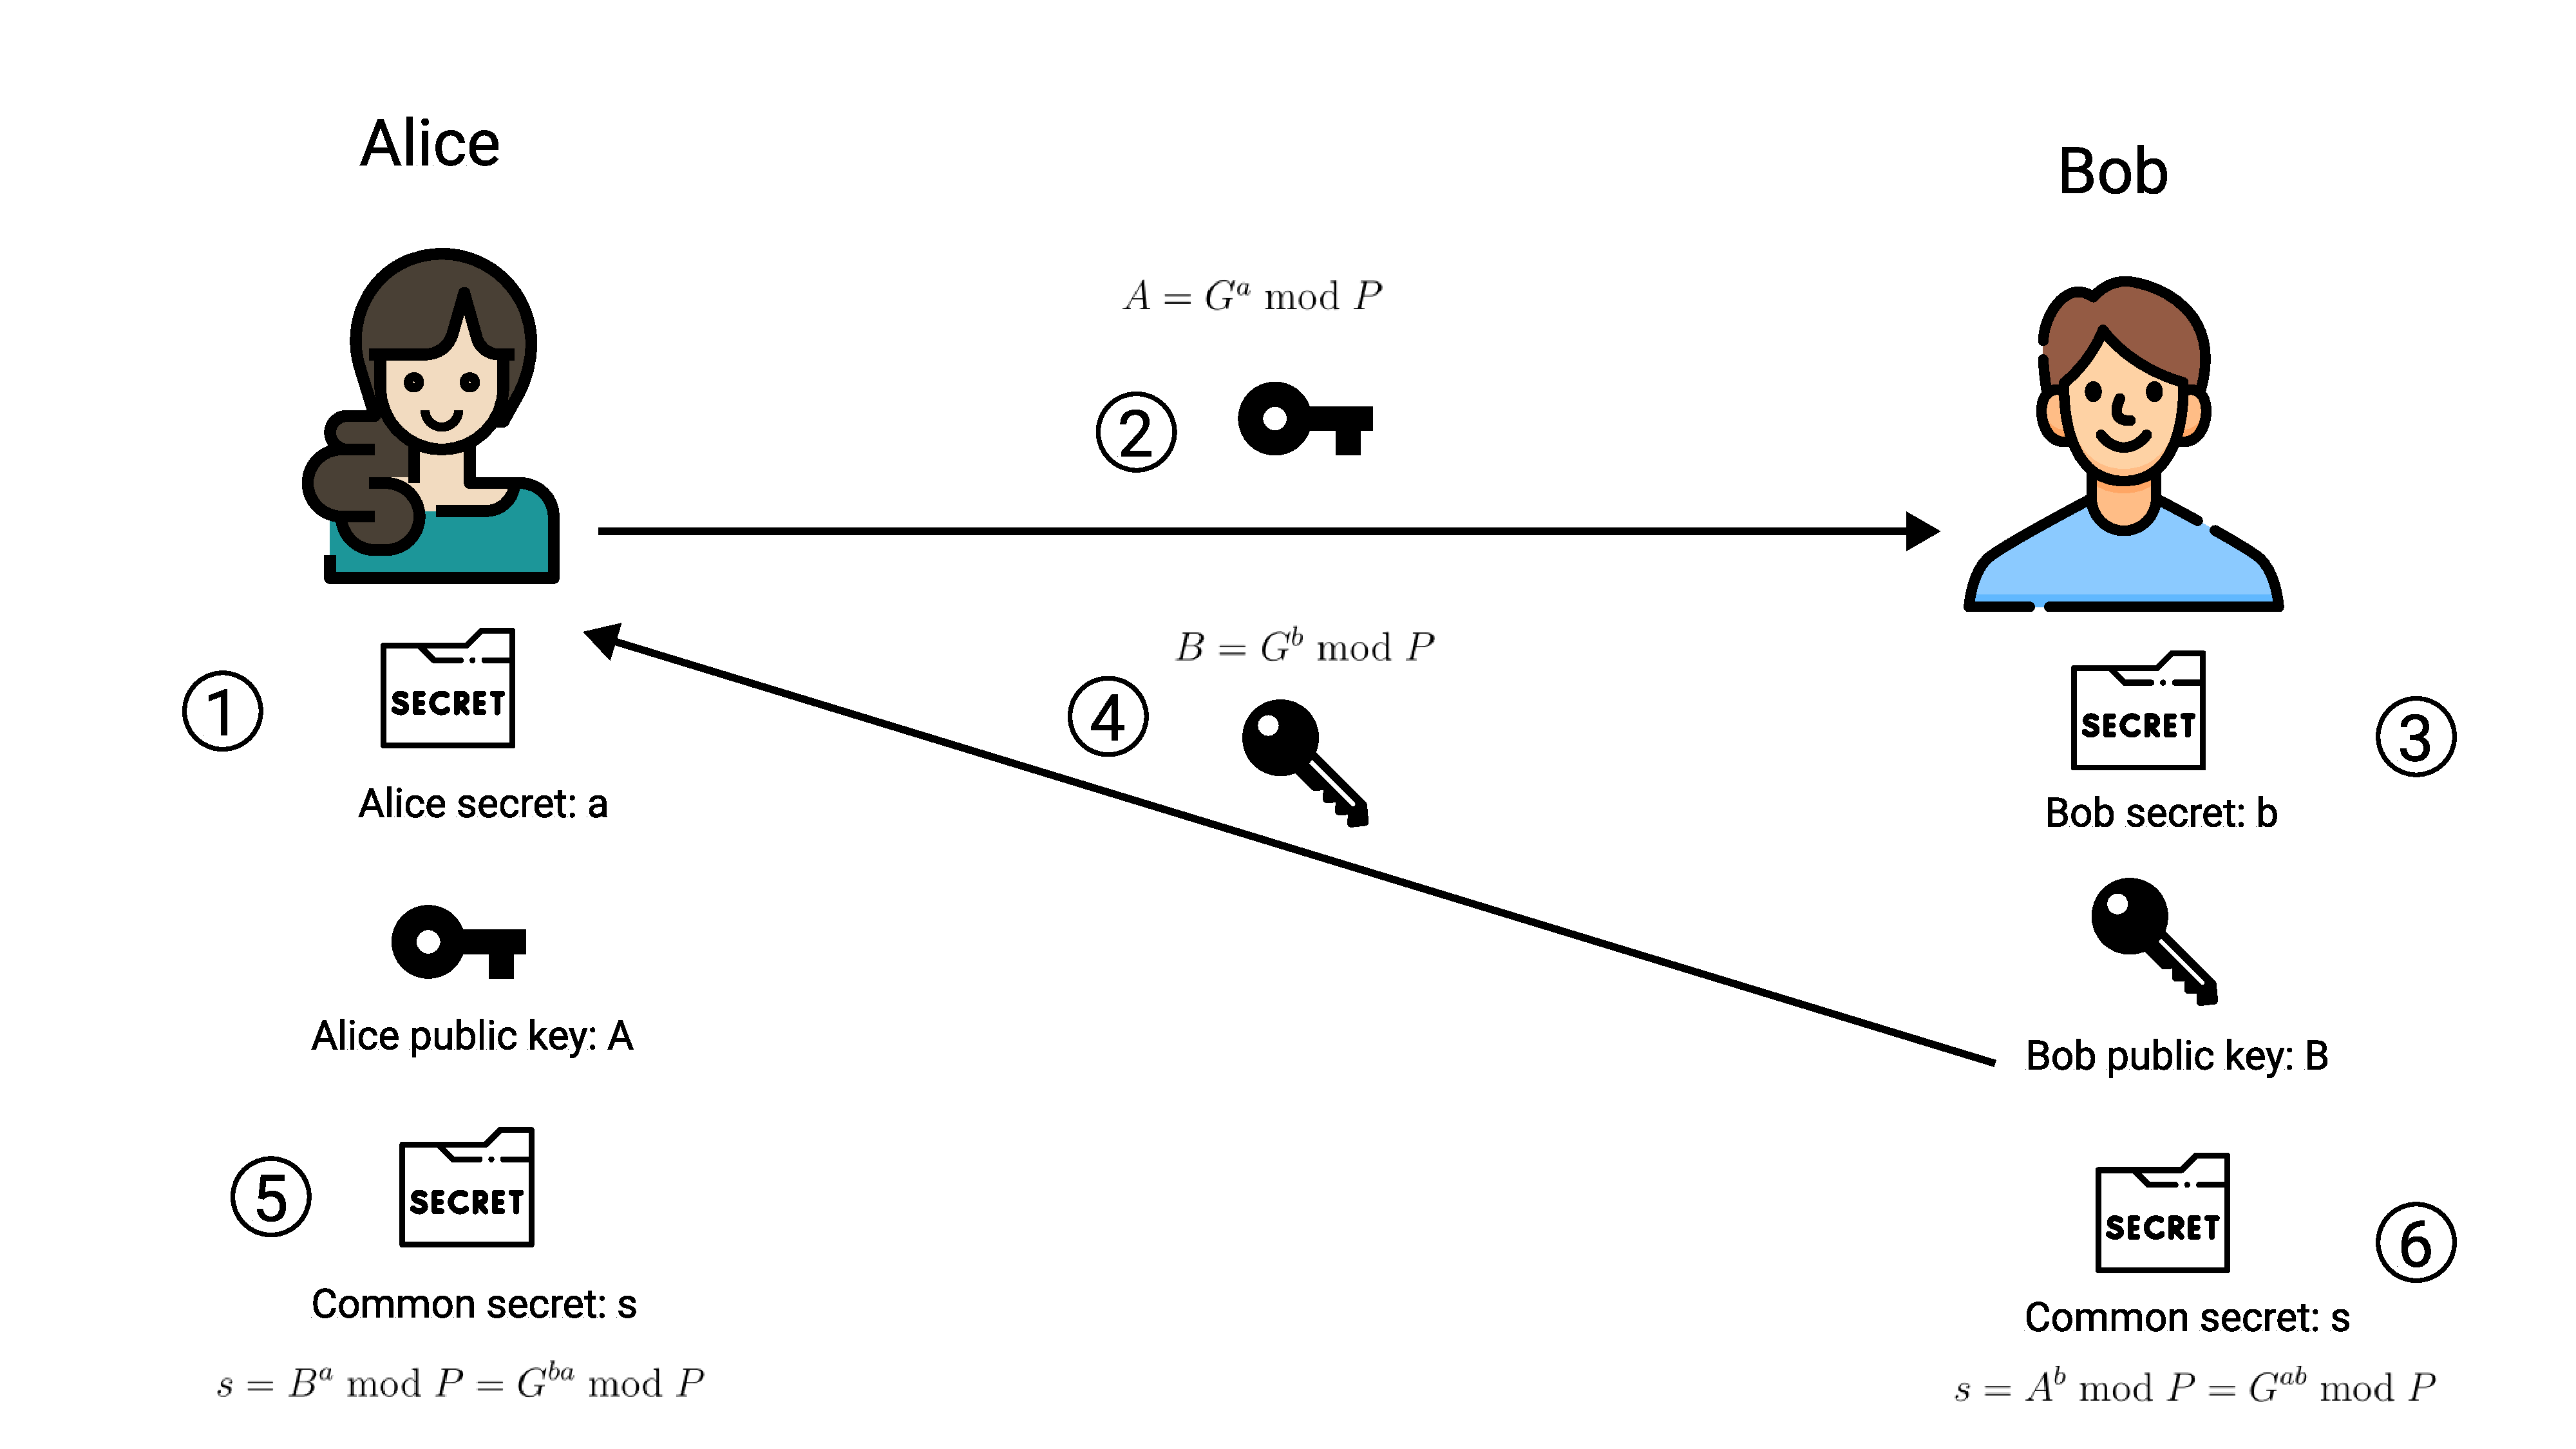
\includegraphics[width=1\textwidth]{Pictures/DH_Key_Exchange}
    ~\caption{Diffie\textendash Hellman key exchange concept diagram.}\label{fig:figure}
\end{figure}